% !Rnw root = learnR.Rnw

%% ---preamble.tex----%% 
%% maxwidth is the original width if it is less than linewidth
%% otherwise use linewidth (to make sure the graphics do not exceed the margin)
\makeatletter
\def\maxwidth{ %
  \ifdim\Gin@nat@width>\linewidth
    \linewidth
  \else
    \Gin@nat@width
  \fi
}
\makeatother

\definecolor{fgcolor}{rgb}{0.345, 0.345, 0.345}

\definecolor{shadecolor}{rgb}{.97, .97, .97}
\definecolor{messagecolor}{rgb}{0, 0, 0}
\definecolor{warningcolor}{rgb}{1, 0, 1}
\definecolor{errorcolor}{rgb}{1, 0, 0}






\marginnote[8pt]{Data objects and functions are two of several types
of objects (others include model objects, formulae, and expressions)
that are available in R.  Users can create and work with such
objects in a user workspace.  All can, if the occasion demands,
be treated as data!}

\noindent
\fbox{\parbox{\linewidth}{{\bf Different types of data objects:}\\[6pt]
\begin{tabular}{ll}
Vectors & These collect together elements of the same mode.\\
& (Possible modes are "logical", "integer", "numeric",\\
& "complex", "character" and "raw")\\[6pt]
Factors & Factors identify category levels in categorical data.\\
        & Modeling functions know how to represent factors.\\
& (Factors do not quite manage to be vectors! Why?)\\[6pt]
Data & A list of columns -- same length; modes may differ. \\
frame & Data frames are a device for organizing data.\\[6pt]
Lists & Lists group together an arbitrary set of objects \\
& (Lists are recursive; elements of lists are lists.)\\[6pt]
\txtt{NA}s & Use \txtt{is.na()} to check for \txtt{NA}s.
\end{tabular}
}}
\vspace*{8pt}

We start this chapter by noting data objects that may appear as
columns of a data frame.

\section{Column Data Objects -- Vectors and Factors}\label{ss:vecDfM}

Column objects is a convenient name for one-dimensional data
structures that can be included as columns in a data frame.
This includes vectors\footnote{Strictly, the vectors that we
  discuss here are \textit{atomic} vectors.  Their elements are not,
  as happens with lists, wrappers for other language objects.},
factors, and dates.

\subsection{Vectors}\label{ss:vector}
Examples of vectors \marginnote{Common vector modes
  are logical, numeric and character. The 4 lines of code create
vectors that are, in order: numeric, numeric, logical, character.} are
\begin{Schunk}
\begin{Sinput}
c(2,3,5,2,7,1)
3:10 # The numbers 3, 4,.., 10
c(TRUE, FALSE, FALSE, FALSE, TRUE, TRUE, FALSE)
c("fig","mango","apple","prune")
\end{Sinput}
\end{Schunk}

Use \txtt{mode()} to show the storage mode of an object, thus:
\begin{Schunk}
\begin{Sinput}
x <- c(TRUE, FALSE, FALSE, FALSE, TRUE, TRUE, FALSE)
mode(x)
\end{Sinput}
\begin{Soutput}
[1] "logical"
\end{Soutput}
\end{Schunk}

The missing value symbol is \txtt{NA}.  Subsection \ref{ss:NA} will
discuss issues that arise when one or more vector elements is an \txtt{NA}.

\subsection*{Subsets of Vectors}
There are four common ways to extract subsets of vectors.

1. Specify the subscripts of elements that are to be extracted:
\begin{Schunk}
\begin{Sinput}
x <- c(3,11,8,15,12)   # Assign to x the values
x[c(2,4)]              # Extract elements 2 and 4
\end{Sinput}
\begin{Soutput}
[1] 11 15
\end{Soutput}
\end{Schunk}
\noindent
Negative numbers may be used to omit elements:\sidenote{Mixing of
  positive and negative subscripts is not allowed.}
\begin{Schunk}
\begin{Sinput}
x <- c(3,11,8,15,12)
x[-c(2,3)]
\end{Sinput}
\begin{Soutput}
[1]  3 15 12
\end{Soutput}
\end{Schunk}

2. Specify a vector of logical values.  \marginnote{Arithmetic
  relations that may be used for extraction of subsets are
  \margtt{>=}, \margtt{==}, \margtt{!=} and \margtt{\%in\%}. The
    first four compare magnitudes, \margtt{==} tests for equality,
    \margtt{!=} tests for inequality, and \margtt{\%in\%} tests
whether any element matches.}  The elements that are
  extracted are those for which the logical value is \txtt{TRUE}.
  Thus suppose we want to extract values of x that are greater than
  10.
\begin{Schunk}
\begin{Sinput}
x>10   # Values are logical (TRUE or FALSE)
\end{Sinput}
\begin{Soutput}
[1] FALSE  TRUE FALSE  TRUE  TRUE
\end{Soutput}
\begin{Sinput}
x[x > 10]
\end{Sinput}
\begin{Soutput}
[1] 11 15 12
\end{Soutput}
\begin{Sinput}
"John" %in% c("Jeff", "Alan", "John")
\end{Sinput}
\begin{Soutput}
[1] TRUE
\end{Soutput}
\end{Schunk}

3. Where elements have names, these can be used to extract elements:
\begin{Schunk}
\begin{Sinput}
altitude <- c(Cambarville=800, Bellbird=300,
              "Allyn River"=300,
              "Whian Whian"=400,
              Byrangery=200, Conondale=400,
              Bulburin=600)
##
## Names can be used to extract elements
altitude[c("Cambarville", "Bellbird")]
\end{Sinput}
\begin{Soutput}
Cambarville    Bellbird 
        800         300 
\end{Soutput}
\end{Schunk}

4. Use \txtt{subset()}, with the vector as the first argument,
and a logical statement that identifies the elements to be
extracted as the second argument. For example:
\begin{Schunk}
\begin{Sinput}
subset(altitude, altitude>400)
\end{Sinput}
\begin{Soutput}
Cambarville    Bulburin 
        800         600 
\end{Soutput}
\end{Schunk}

\subsection{Factors}\label{ss:factors}
\marginnote{Factors are an economical way to store vectors of
  repetitive text strings. By default, when a vector of text strings
  becomes a column in a data frame, it is incorporated as a factor.}

Factors are column objects whose elements are integer values 1, 2,
\ldots, $k$, where $k$ is the number of levels.  They are
distinguished from integer vectors by having the class \txtt{factor}
and a \txtt{levels} attribute.

For example, create a character vector \txtt{fruit}, thus:
\begin{Schunk}
\begin{Sinput}
fruit <- c("fig","mango","apple","plum", "fig")
\end{Sinput}
\end{Schunk}
This might equally well be stored as a factor, thus:
\begin{Schunk}
\begin{Sinput}
fruitfac <- factor(fruit)
\end{Sinput}
\end{Schunk}

Internally, the factor is stored\marginnote{Thus 1 is interpreted
as \margtt{"apple"}; 2:\margtt{"fig"};
3:\margtt{"mango"}; 4:\margtt{"plum"}.}
as the integer vector 2, 3, 1, 4, 2. These numbers are
interpreted according to the attributes table:\\[2mm]
\begin{tabular}{|cccc|}
\hline
1 & 2 & 3 & 4\\
\verb!"apple"! & \verb!"fig"! & \verb!"mango"! & \verb!"plum"!\\
\hline
\end{tabular}
\vspace*{8pt}

\noindent
By default, the levels are taken in alphanumeric order.

The function \txtt{factor()}, with the \txtt{levels} argument
specified, can be used both to specify the order of levels when the
factor is created, or to make a later change to the
order.\sidenote{Where counts are tabulated by factor level, or
  \textit{lattice} or other graphs have one panel per factor level,
  these are in order of the levels.}  For example, the following
orders levels according to stated glycemic index:
\begin{Schunk}
\begin{Sinput}
glycInd <- c(apple=40, fig=35, mango=55, plum=25)
## Take levels in order of stated glycInd index
fruitfac <- factor(fruit,
                   levels=names(sort(glycInd)))
levels(fruitfac)
\end{Sinput}
\begin{Soutput}
[1] "plum"  "fig"   "apple" "mango"
\end{Soutput}
\begin{Sinput}
unclass(fruitfac)  # Examine stored values
\end{Sinput}
\begin{Soutput}
[1] 2 4 3 1 2
attr(,"levels")
[1] "plum"  "fig"   "apple" "mango"
\end{Soutput}
\end{Schunk}

Incorrect spelling of the level names generates missing values, for
the level that was mis-spelled.  Use the \txtt{labels} argument if you
wish to change the level names, but be careful to ensure that the
label names are in the correct order.
\begin{marginfigure}[-36pt]
Mis-spelt name, example:
\begin{Schunk}
\begin{Sinput}
trt <- c("A","A","Control")
trtfac <- factor(trt,
  levels=c("control","A"))
table(trtfac)
\end{Sinput}
\begin{Soutput}
trtfac
control       A 
      0       2 
\end{Soutput}
\end{Schunk}
\end{marginfigure}

In most places where the context seems to demand it, the integer levels
are translated into text strings, thus:
\begin{Schunk}
\begin{Sinput}
fruit <- c("fig","mango","apple", "plum","fig")
fruitfac <- factor(fruit)
fruitfac == "fig"
\end{Sinput}
\begin{Soutput}
[1]  TRUE FALSE FALSE FALSE  TRUE
\end{Soutput}
\end{Schunk}

Section \ref{ss:facs} has detailed examples of the use of factors
in model formulae.

\subsection*{Ordered factors}
In addition to factors, note the existence of ordered factors, created
using the function \txtt{ordered()}.  For ordered factors, the order
of levels implies a relational ordering.  For example:
\begin{Schunk}
\begin{Sinput}
windowTint <- ordered(rep(c("lo","med","hi"), 2),
                      levels=c("lo","med","hi"))
windowTint
\end{Sinput}
\begin{Soutput}
[1] lo  med hi  lo  med hi 
Levels: lo < med < hi
\end{Soutput}
\begin{Sinput}
sum(windowTint > "lo")
\end{Sinput}
\begin{Soutput}
[1] 4
\end{Soutput}
\end{Schunk}

\subsection*{Subsetting of factors}

Consider the factor \txtt{fruitfac} that was created earlier:
\begin{Schunk}
\begin{Sinput}
fruitfac <- factor(c("fig","mango","apple","plum", "fig"))
\end{Sinput}
\end{Schunk}
We can remove elements with levels \txtt{fig} and \txtt{plum} thus:
\begin{Schunk}
\begin{Sinput}
ff2 <- fruitfac[!fruitfac %in% c("fig","plum")]
ff2
\end{Sinput}
\begin{Soutput}
[1] mango apple
Levels: apple fig mango plum
\end{Soutput}
\begin{Sinput}
table(ff2)
\end{Sinput}
\begin{Soutput}
ff2
apple   fig mango  plum 
    1     0     1     0 
\end{Soutput}
\end{Schunk}
The levels \txtt{fig} and \txtt{plum} remain, but with
the table showing 0 values for these levels.  Use the function
\txtt{droplevels()} to remove levels that are not present in
the data:
\begin{marginfigure}
Note also:
\begin{Schunk}
\begin{Sinput}
table(droplevels(ff2))
\end{Sinput}
\begin{Soutput}

apple mango 
    1     1 
\end{Soutput}
\end{Schunk}
\end{marginfigure}
\begin{Schunk}
\begin{Sinput}
droplevels(ff2)
\end{Sinput}
\begin{Soutput}
[1] mango apple
Levels: apple mango
\end{Soutput}
\end{Schunk}

\subsection*{Why is a factor not a vector?}
Two factors \marginnote{Vectors can be concatenated (joined). Two or
  mare factors can be sensibly concatenated only if they have
identical levels vectors.}  that
have different levels vectors are different types of object.  Thus,
formal concatenation of factors with different levels vectors is
handled by first coercing both factors to integer vectors.  The
integer vector that results is not, in most circumstances, meaningful
or useful.

\subsection{Missing Values, Infinite Values and NaNs}\label{ss:NA}

Any arithmetic or logical operation with \txtt{NA} generates an
\marginnote{Failure to understand the rules for calculations with
  \txtt{NA}s can lead to unwelcome surprises.}
\txtt{NA}. The consequences are more far-reaching than might be
immediately obvious.  Use \txtt{is.na()} to test for a missing value:
\begin{Schunk}
\begin{Sinput}
is.na(c(1, NA, 3, 0, NA))
\end{Sinput}
\begin{Soutput}
[1] FALSE  TRUE FALSE FALSE  TRUE
\end{Soutput}
\end{Schunk}

An expression such as \txtt{c(1, NA, 3, 0, NA) == NA} returns a vector of
\txtt{NA}s, and cannot be used to test for missing values.
\begin{Schunk}
\begin{Sinput}
c(1, NA, 3, 0, NA) == NA
\end{Sinput}
\begin{Soutput}
[1] NA NA NA NA NA
\end{Soutput}
\end{Schunk}
\noindent
As the value is unknown, it might or might not be equal to 1, or to another
\txtt{NA}, or to 3, or to 0.

Note that different functions handle \txtt{NA}s in\marginnote{The
  modeling function \txtt{lm()} accepts any of the arguments
  \txtt{na.action=na.omit} (omit), \txtt{na.action=na.exclude} (omit
  \txtt{NA}s when fitting; replace by \txtt{NA}s
   when fitted values and residuals are calculated), and
  \txtt{na.action=na.fail}.}  different ways.  Functions such as
\txtt{mean()} and \txtt{median()} accept the argument
\txtt{na.rm=TRUE}, which causes observations that have \txtt{NA}s to
be ignored.  The \txtt{plot()} function omits \txtt{NA}s, infinities
and \txtt{NaN}s. For use of \txtt{lowess()} to put a smooth curve
through the plot, \txtt{NA}s must first be removed.  By default,
\txtt{table()} ignores \txtt{NA}s.

Problems with missing values are a common reason why calculations
fail. Infinite values and \txtt{NaN}s are a further potential source
of difficulty.

\subsection*{\texttt{Inf} and \texttt{NaN}}

The expression \txtt{1/0} returns \txtt{Inf}.\marginnote{Note that
\txtt{sqrt(-1+0i)} returns \txtt{0+1i}. R distinguishes between
the real number \txtt{-1} and the complex number \txtt{-1+0i}.}
The expression \txtt{log(0)} returns \txtt{-Inf},
i.e., smaller than any real number. The expressions \txtt{0/0} and
\txtt{log(-1)} both return \txtt{NaN}.

\subsection*{\txtt{NA}s in subscripts?}

It is best to ensure that \txtt{NA}s do not appear, when there
is an assignment, in subscript expressions on either side of the
expression.

\section{Data Frames, Matrices, Arrays and Lists}\label{sec:dframes}

\marginnote{Data frames with all columns numeric can sometimes be
  handled in the same way as matrices.  In other cases, a different
  syntax may be needed, or conversion from one to the other.
  Proceed with care!}
\paragraph{Data frames:} Data frames are lists of column objects.
The requirement that all
of the column objects have the same length gives data frames a row
by column rectangular structure.  Different columns can have different
column classes --- commonly numeric or character or factor or logical
or date.

\paragraph{Matrices -- vectors with a Dimension:}
\marginnote[8pt]{Internally, matrices are stored as one long vector
  in which the columns are stacked one above the other.  The first
  element in the dimension attribute gives the number of rows in each
  column.}
When printed, matrices appear in a row by column layout in which all
elements have the same mode -- commonly numeric or character or
logical.

\paragraph{Arrays and tables:} Matrices are two-dimensional arrays.
Arrays more generally can have an arbitrary number of dimensions.
Tables have a structure that is identical to that of arrays.

The data frame \txtt{travelbooks} will feature in the subsequent
discussion.  Look back to Section \ref{sec:input} to see how it can be
entered.



\subsection{Data frames versus matrices and tables}\label{ss:df-mat}

\marginnote[12pt]{Computations that can be performed with matrices are
  typically much faster than their equivalents with data frames.  See
  Section \ref{sec:large-dset}.}  Modeling functions commonly return
larger numeric objects as matrices rather than data frames. The
principal components function \margtt{prcomp()} returns scores as a
matrix, as does the linear discriminant analysis function
\margtt{lda()} from the {\em MASS} package.

Functions are available to convert data frames into matrices, and vice
versa. For example:
\begin{Schunk}
\begin{Sinput}
travelmat <- as.matrix(travelbooks[, 1:4])
  # From data frame to matrix
newtravelbooks <- as.data.frame(travelmat)
  # From matrix to data frame
\end{Sinput}
\end{Schunk}

\enlargethispage{24pt}

In comparing data frames with matrices, note that:
\begin{itemizz}
\item Both for data frames and for matrices or two-way tables,
the function \txtt{dim()} returns number of rows by number of columns,
thus:
\begin{marginfigure}
Alternatively, do:
\begin{Schunk}
\begin{Sinput}
attr(travelmat, "dim")
\end{Sinput}
\begin{Soutput}
[1] 6 4
\end{Soutput}
\end{Schunk}
\end{marginfigure}
\begin{Schunk}
\begin{Sinput}
travelmat <- as.matrix(travelbooks[, 1:4])
dim(travelmat)
\end{Sinput}
\begin{Soutput}
[1] 6 4
\end{Soutput}
\end{Schunk}
\item \marginnote[12pt]{A data frame is a list of columns.
   The function \txtt{length()} returns the list length.}
  For a matrix, \txtt{length()} returns the number of elements.
For a data frame it returns the number of columns.
\begin{Schunk}
\begin{Sinput}
c(dframelgth=length(travelbooks),
  matlgth=length(travelmat))
\end{Sinput}
\begin{Soutput}
dframelgth    matlgth 
         6         24 
\end{Soutput}
\end{Schunk}
\item The notation that uses single square left and right brackets
to extract subsets of data frames, introduced in Section \ref{sec:df}
works in just the same way with matrices.  For example
\begin{Schunk}
\begin{Sinput}
travelmat[, 4]
travelmat[, "weight"]
travelmat[, 1:3]
travelmat[2,]
\end{Sinput}
\end{Schunk}
Negative indices can be used to omit rows and/or columns.
\item Use of the subscript notation to extract a row from a data
frame returns a data frame, whereas extraction of a column yields a
column vector.  Thus:
\begin{itemizz}
\item
\marginnote[12pt]{Use \margtt{unlist(travelbooks[6, ])} to turn row
from the data frame into a vector. All elements are coerced to a
common mode, in this case numeric.  Thus the final element becomes
1.0 (the code that is stored), rather than \margtt{Guide} which was
the first level of the factor \margtt{type}.}
Extraction of a row from a data frame, for example
  \txtt{travelbooks["Canberra - The Guide", ]}
  or \txtt{travelbooks[6, ]}, yields a data frame,
  i.e., a special form of list.
\item \verb!travelbooks$volume! (equivalent to \txtt{travelbooks[,1]}
or \txtt{travelbooks[,"volume"]})) is a vector.
\end{itemizz}
\item For either a data frame or a matrix, the function
\txtt{rownames()} can be used to extract row names, and the
function \txtt{colnames()} to extract column names.  For
data frames, \txtt{row.names()} is an alternative to
\txtt{rownames()}, while \txtt{names()} is an alternative to
\txtt{colnames()}.
\end{itemizz}

Note also a difference in the mechanisms for adding columns.  The
following adds new columns \txtt{area} (area of page), and
\txtt{density} (\txtt{weight} to \txtt{volume} ratio) to the data
frame \txtt{travelbooks}:
\begin{Schunk}
\begin{Sinput}
travelbooks$area <- with(travelbooks, width*height)
travelbooks$density <- with(travelbooks,
                            weight/volume)
names(travelbooks)   # Check column names
\end{Sinput}
\begin{Soutput}
[1] "thickness" "width"     "height"    "weight"    "volume"    "type"     
[7] "area"      "density"  
\end{Soutput}
\end{Schunk}
Columns are added to the data frame as necessary.

For matrices, use \txtt{cbind()}, which can also be used for data
frames, to bind in new columns.
\enlargethispage{12pt}

\subsection{Inclusion of character vectors in data frames}
When data frames are created, whether by use of
\txtt{read.table()} or another such function to input data from a
file, or by use of the function \txtt{data.frame()} to
join columns of data together into a data frame, character vectors are
converted into factors.  Thus, the final column (\txtt{type}) of
\txtt{travelbooks} became, by default, a factor.\footnote{This assumes
that the global option \txtt{stringsAsFactors} is \txtt{FALSE}.
To check, interrogate {\footnotesize \txtt{options()\$stringsAsFactors}.}}
%$
To prevent such type conversions, specify \txtt{stringsAsFactors=FALSE}
in the call to \txtt{read.table()} or \txtt{data.frame()}.

\subsection{Factor columns in data frame subsets}

The data frame \txtt{ais} ({\em DAAG}) has physical charateristics
of athletes, divided up thus between ten different sports:
\begin{fullwidth}
\begin{minipage}[t]{\linewidth}

\begin{Schunk}
\begin{Sinput}
with(ais, table(sport))
\end{Sinput}
\begin{Soutput}
sport
 B_Ball   Field     Gym Netball     Row    Swim  T_400m T_Sprnt  Tennis 
     25      19       4      23      37      22      29      15      11 
 W_Polo 
     17 
\end{Soutput}
\end{Schunk}

\end{minipage}
\end{fullwidth}

Figure \ref{ss:lat-gph} in Subsection \ref{fig:lattice-ais} limits the
data to swimmers and rowers. For this, at the same time removing all
levels except \txtt{Row} and \txtt{Swim} from the factor \txtt{sport},
do:
\marginnote[17pt]{If redundant levels were left in place, the graph
would show empty panels for each such level.}
\begin{Schunk}
\begin{Sinput}
rowswim <- with(ais, sport %in% c("Row", "Swim"))
aisRS <- droplevels(subset(ais, rowswim))
xtabs(~sport, data=aisRS)
\end{Sinput}
\begin{Soutput}
sport
 Row Swim 
  37   22 
\end{Soutput}
\end{Schunk}
Contrast the above with:
\begin{fullwidth}

\begin{Schunk}
\begin{Sinput}
xtabs(~sport, data=subset(ais, rowswim))
\end{Sinput}
\begin{Soutput}
sport
 B_Ball   Field     Gym Netball     Row    Swim  T_400m T_Sprnt  Tennis 
      0       0       0       0      37      22       0       0       0 
 W_Polo 
      0 
\end{Soutput}
\end{Schunk}

\end{fullwidth}

\subsection{Handlng rows that include missing values}
The function \txtt{na.omit()} omits rows that contain one
or more missing values. The argument may be a data frame or a
matrix. The function \txtt{complete.cases()} identifies
such rows. Thus:
\begin{Schunk}
\begin{Sinput}
test.df <- data.frame(x=c(1:2,NA), y=1:3)
test.df
\end{Sinput}
\begin{Soutput}
   x y
1  1 1
2  2 2
3 NA 3
\end{Soutput}
\begin{Sinput}
## complete.cases()
complete.cases(test.df)
\end{Sinput}
\begin{Soutput}
[1]  TRUE  TRUE FALSE
\end{Soutput}
\begin{Sinput}
## na.omit()
na.omit(test.df)
\end{Sinput}
\begin{Soutput}
  x y
1 1 1
2 2 2
\end{Soutput}
\end{Schunk}

\subsection{Arrays --- some further details}
\marginnote[12pt]{Tables, which will be the subject of the next subsection, have
a very similar structure to arrays.}

A matrix is a two-dimensional array.  More generally, arrays can
have an arbitrary number of dimensions.

\subsection*{Removal of the dimension attribute}

The dimension attribute of a matrix or array can be changed or
removed, thus:
\begin{fullwidth}

\begin{Schunk}
\begin{Sinput}
travelvec <-  as.matrix(travelbooks[, 1:4])
dim(travelvec) <- NULL  # Columns of travelmat are stacked into one
                        # long vector
travelvec
\end{Sinput}
\begin{Soutput}
 [1]    1.3    3.9    1.2    2.0    0.6    1.5   11.3   13.1   20.0   21.1
[11]   25.8   13.1   23.9   18.7   27.6   28.5   36.0   23.4  250.0  840.0
[21]  550.0 1360.0  640.0  420.0
\end{Soutput}
\begin{Sinput}
  # as(travelmat, "vector") is however preferable
\end{Sinput}
\end{Schunk}

\end{fullwidth}

Note again that the \txtt{\$} notation, used with data frames
  and other list objects to reference the contents of list elements, is
  not relevant to matrices.

\subsection{Lists}\label{sec:df-lists}

A list \marginnote{Elements of lists are themselves lists.
Distinguish \margtt{rcanberra[4]}, which is a sub-list
and therefore a list, from \margtt{rcanberra[[4]]} which extracts the
contents of the fourth list element.} is a collection of arbitrary
objects. As noted above, a data frame is a specialized form of
list. Consider for example the list
\begin{Schunk}
\begin{Sinput}
rCBR <- list(society="ssai", branch="Canberra",
             presenter="John",
             tutors=c("Emma", "Chris", "Frank"))
\end{Sinput}
\end{Schunk}

First, extract list length and list names:
\begin{Schunk}
\begin{Sinput}
length(rCBR)      # rCBR has 4 elements
names(rCBR)
\end{Sinput}
\end{Schunk}

\begin{Schunk}
\begin{Soutput}
[1] 4
\end{Soutput}
\begin{Soutput}
[1] "society"   "branch"    "presenter" "tutors"   
\end{Soutput}
\end{Schunk}

The following extracts the 4th list element:
\begin{Schunk}
\begin{Sinput}
rCBR[4]           # Also a list,  name is 'tutors'
\end{Sinput}
\begin{Soutput}
$tutors
[1] "Emma"  "Chris" "Frank"
\end{Soutput}
\end{Schunk}

Alternative ways to extract the contents of the 4$^{th}$ element are:
\marginnote[12pt]{List elements can be accessed by name.
  Thus, to extract the contents of the 4th list element, alternatives
to \margtt{rcanberra[[4]]} are \margtt{rcanberra[["tutors"]]} or
\margtt{rcanberra\$tutors}.}
\begin{Schunk}
\begin{Sinput}
rCBR[[4]]         # Contents of 4th list element
\end{Sinput}
\begin{Soutput}
[1] "Emma"  "Chris" "Frank"
\end{Soutput}
\begin{Sinput}
rCBR$tutors       # Equivalent to rCBR[["tutors"]]
\end{Sinput}
\begin{Soutput}
[1] "Emma"  "Chris" "Frank"
\end{Soutput}
\end{Schunk}

\subsection*{Model objects are lists}
As noted in Subsection \ref{ss:modobj}, the various R modeling
\marginnote{Recall again, also, that data frames are a specialized
  form of list, with the restriction that all columns must all have
  the same length.}  functions all return their own particular type of
model object, either a list or as an S4 object.

\section{Functions}
\noindent
\fbox{\parbox{\textwidth}{
\textbf{Different Kinds of Functions:}\\[4pt]
\begin{tabular}{ll}
  Generic & The 'class' of the function argument determines the\\
          & action taken. E.g., \txtt{print()}, \txtt{plot()}, \txtt{summary()}\\[6pt]
  Modeling  & For example, \txtt{lm()} fits \textit{linear} models.\\
            & Output may be stored in a model object.\\[6pt]
  Extractor & These extract information from model objects.\\
  &  Examples include \txtt{summary()}), \txtt{coef()}),\\
  & \txtt{resid()}), and \txtt{fitted()}\\[6pt]
  User & Use, e.g., to automate and document computations\\[6pt]
  Anonymous & These are user functions that are defined at the\\
 & point of use, and do not need a name.
\end{tabular}
}}
\vspace*{6pt}

The above list is intended to include the some of the most important
types of function.  These categories may overlap.

The language that R implements has many of the features
of\marginnote{Functions for working with dates are discussed in
  Section \ref{ss:dates} immediately following.}  a
functional language. Functions have accordingly featured throughout
the earlier discussion.  Here will be noted functions that are
commonly important.

\subsection{Built-In Functions}\label{ss:built-in}

\subsection*{Common useful functions}

\begin{fullwidth}
\begin{verbcode}
## Use with any R object as argument
print()           # Prints a single R object
length()          # Number of elements in a vector or of a list

## Concatenate and print R objects [does less coercion than print()]
cat()             # Prints multiple objects, one after the other

## Use with a numeric vector argument
mean()            # If argument has NA elements, may want na.rm=TRUE
median()          # As for mean(), may want na.rm=TRUE
range()           # As for mean(), may want na.rm=TRUE
unique()          # Gives the vector of distinct values
diff()            # Vector of first differences
                  # N. B. diff(x) has one less element than x
cumsum()          # Cumulative sums, c.f., also, cumprod()

## Use with an atomic vector object
sort()            # Sort elements into order, but omitting NAs
order()           # x[order(x)] orders elements of x, with NAs last
rev()             # reverse the order of vector elements
any()             # Returns TRUE if there are any missing values
as()              # Coerce argument 1 to class given by argument 2
                  # e.g. as(1:6, "factor")
is()              # Is argument 1 of class given by argument 2?
                  # is(1:6, "factor") returns FALSE
                  # is(TRUE, "logical") returns TRUE
is.na()           # Returns TRUE if the argument is an NA

## Information on an R object
str()             # Information on an R object
args()            # Information on arguments to a function
mode()            # Gives the storage mode of an R object
                  # (logical, numeric, character, . . ., list)

## Create a vector
numeric()         # numeric(5) creates a numeric vector, length 5,
                  # all elements 0.
                  # numeric(0) (length 0) is sometimes useful.
character()       # Create character vector; c.f. also logical()
\end{verbcode}
\end{fullwidth}

The function \txtt{mean()}, and a number of other functions, takes the
argument \txtt{na.rm=TRUE}; i.e., remove \txtt{NA}s, then proceed with
the calculation. For example
\begin{Schunk}
\begin{Sinput}
mean(c(1, NA, 3, 0, NA), na.rm=T)
\end{Sinput}
\begin{Soutput}
[1] 1.333
\end{Soutput}
\end{Schunk}

Note that the function \txtt{as()} has, at present, no method for
coercing a matrix to a data frame. For this, use
\txtt{as.data.frame()}.

\subsection*{Functions in different packages with the same name}
For example, as well as {\em lattice} function \txtt{dotplot()}
the graphics package has a defunct function \txtt{dotplot()}.
To be sure of getting the {\em lattice} function {\em dotplot()},
refer to it as \txtt{lattice::dotplot}.


\subsection{Functions for data summary and/or manipulation}
\marginnote[-12pt]{For
data manipulation, note:
\begin{itemizz}
\item[-] the apply family of functions (Subsection \ref{ss:apply}).
\item[-] data manipulation functions in the \textit{reshape2} and
\textit{plyr} packages (Chapter \ref{ch:manip}).
\end{itemizz}}

\subsection{Functions for creating and working with tables}\label{sec:tab}

\subsection{Tables of Counts}

Use either \txtt{table()} or \txtt{xtabs()} to make a table of
counts. Use \txtt{xtabs()} for cross-tabulation, i.e., to determine
totals of numeric values for each table category.

\subsection*{The \texttt{table()} function}\label{ss:table}
For use of \txtt{table()}, specify one vector of values (often a
factor) for each table margin that is required.  For example:
\begin{Schunk}
\begin{Sinput}
library(DAAG)        # possum is from DAAG
with(possum, table(Pop, sex))
\end{Sinput}
\begin{Soutput}
       sex
Pop      f  m
  Vic   24 22
  other 19 39
\end{Soutput}
\end{Schunk}

\subsection*{NAs in tables}

By default, \txtt{table()} ignores NAs. To show information on
\txtt{NA}s, specify \txtt{exclude=NULL}, thus:
\begin{Schunk}
\begin{Sinput}
library(DAAG)
table(nswdemo$re74==0, exclude=NULL)
\end{Sinput}
\begin{Soutput}

FALSE  TRUE  <NA> 
  119   326   277 
\end{Soutput}
\end{Schunk}


\subsection*{The \texttt{xtabs()} function}
This more flexible alternative to \txtt{table()} uses a table
formula to specify the margins of the table:
\begin{Schunk}
\begin{Sinput}
xtabs(~ Pop+sex, data=possum)
\end{Sinput}
\begin{Soutput}
       sex
Pop      f  m
  Vic   24 22
  other 19 39
\end{Soutput}
\end{Schunk}

\marginnote[12pt]{Manipulations with data frames are in general
conceptually simpler than manipulations with tables. For tables
that are not unreasonably large, it is in general a good strategy
to first convert the table to a data frame and make that the
starting point for further calculations.}
A column of frequencies can be specified on the left hand side of the
table formula. In order to demonstrate this, the three-way table
\txtt{UCBAdmissions} ({\em datasets} package) will be converted into
its data frame equivalent.  Margins in the table become columns in
the data frame:
\begin{Schunk}
\begin{Sinput}
UCBdf <- as.data.frame.table(UCBAdmissions)
head(UCBdf, n=3)
\end{Sinput}
\begin{Soutput}
     Admit Gender Dept Freq
1 Admitted   Male    A  512
2 Rejected   Male    A  313
3 Admitted Female    A   89
\end{Soutput}
\end{Schunk}

The following then forms a table of total admissions and rejections
in each department:
\begin{Schunk}
\begin{Sinput}
xtabs(Freq ~  Admit+Dept, data=UCBdf)
\end{Sinput}
\begin{Soutput}
          Dept
Admit        A   B   C   D   E   F
  Admitted 601 370 322 269 147  46
  Rejected 332 215 596 523 437 668
\end{Soutput}
\end{Schunk}


\subsection*{Information on data objects}

The function \txtt{str()} gives basic information on the data object that
is given as argument.
\begin{Schunk}
\begin{Sinput}
library(DAAG)
str(possumsites)
\end{Sinput}
\begin{Soutput}
'data.frame':	7 obs. of  3 variables:
 $ Longitude: num  146 149 151 153 153 ...
 $ Latitude : num  -37.5 -37.6 -32.1 -28.6 -28.6 ...
 $ altitude : num  800 300 300 400 200 400 600
\end{Soutput}
\end{Schunk}

\subsection{Utility functions}
\begin{fullwidth}
\begin{verbcode}
dir()             # List files in the working or other specified directory
sessionInfo()     # Print version numbers for R and for attached packages
system.file()     # By default, show path to 'package="base"'
R.home()          # Path to R home directory
.Library          # Path to the default library
.libPaths()       # Get/set paths to library directories
\end{verbcode}
\end{fullwidth}
Section \ref{ch:sys} has further details.

\subsection{User-defined functions}
\marginnote[8pt]{Note also that functions can be defined at the point of
  use.  Such functions do not need a name, and are called anonymous
  functions.  Section \ref{ss:table} has an example.}
The function \txtt{mean()} calculates means, The function \txtt{sd()}
calculates standard deviations. Here is a function that calculates
mean and standard deviation at the same time:
\begin{Schunk}
\begin{Sinput}
mean.and.sd <- function(x){
    av <- mean(x)
    sdev <- sd(x)
    c(mean=av, sd = sdev)   # return value
}
\end{Sinput}
\end{Schunk}
The parameter \txtt{x} is the argument that the user must supply.
The body of the function is enclosed between curly braces. The value
that the function returns is given on its final line. Here the return
value is a vector that has two named elements.

The following calculates the mean and standard deviation of
heterozygosity estimates for seven different \textit{Drosophila}
species.\footnote{Data are from Lewontin, R. 1974. \textit{The Genetic
    Basis of Evolutionary Change}.}
\begin{Schunk}
\begin{Sinput}
hetero <- c(.43,.25,.53,.47,.81,.42,.61)
mean.and.sd(hetero)
\end{Sinput}
\begin{Soutput}
  mean     sd 
0.5029 0.1750 
\end{Soutput}
\end{Schunk}

It is useful to give the function argument a default value, so that it can be
run without user-supplied parameters, in order to see what it does. A
possible choice is a set of random normal numbers, perhaps generated
using the \txtt{rnorm()} function.
\enlargethispage{24pt}
Here is a revised function definition.\marginnote{Note that a
  different set of random numbers will be returned, giving a different
  mean and SD, each time that the function is run with its default
  argument.}  Because the function body has been reduced to a single
line, the curly braces are not needed.
\begin{Schunk}
\begin{Sinput}
mean.and.sd <- function(x = rnorm(20))
                 c(mean=mean(x), sd=sd(x))
mean.and.sd()
\end{Sinput}
\begin{Soutput}
   mean      sd 
0.00408 0.95165 
\end{Soutput}
\begin{Sinput}
mean.and.sd()
\end{Sinput}
\begin{Soutput}
 mean    sd 
0.383 1.294 
\end{Soutput}
\end{Schunk}

\subsection{The \texttt{apply} family of functions}\label{ss:apply}

\marginnote[8pt]{For the \margtt{apply} family of functions, specify
  as the \margtt{FUN} argument any function that will not generate an
  error.  Obviously, \margtt{log("Hobart")} is not allowed!}
\marginnote[6pt]{Note also the function \margtt{tapply()}, which will
  not be discussed here.}
\fbox{\parbox{\linewidth}{{\bf \txtt{apply()}, \txtt{sapply()} and friends }\\[4pt]
\begin{tabular}{ll}
\txtt{apply()} & Use \txtt{apply()} to apply a function across rows\\
& or columns of a matrix (or data frame)\\[6pt]
\txtt{sapply()} & \txtt{sapply()} and \txtt{lapply()} apply functions
in\\
\& friends &  parallel across columns of a data frame,  or across\\
& elements of a list, or across elements of a vector.\\
\end{tabular}
}}

\paragraph{\txtt{apply()}:}
\marginnote[12pt]{If used with a data
frames, the data frame is first coerced to \txtt{matrix}.}
The function \txtt{apply()} is intended for use with matrices or, more
generally, with arrays.
It has three mandatory arguments, a matrix or data frame, the dimension
(1 for rows; 2 for columns) or dimensions, and a function that will be
applied across that dimension of the matrix or data frame.

Here is an example:
\begin{marginfigure}[30pt]
Code that will input \margtt{molclock1}:
\begin{Schunk}
\begin{Sinput}
library(DAAG)
datafile("molclock1")
molclock <-
  read.table("molclock1.txt")
\end{Sinput}
\end{Schunk}
\end{marginfigure}

\begin{Schunk}
\begin{Sinput}
apply(molclock, 2, range)
\end{Sinput}
\end{Schunk}

The following tabulates admissions, in the three-way table
\txtt{UCBAdmissions}, according to \txtt{sex}:
\begin{Schunk}
\begin{Sinput}
apply(UCBAdmissions, c(1,2), sum)
\end{Sinput}
\begin{Soutput}
          Gender
Admit      Male Female
  Admitted 1198    557
  Rejected 1493   1278
\end{Soutput}
\end{Schunk}

\paragraph{\txtt{sapply()} and \txtt{lapply()}:}
\marginnote[12pt]{\noindent
  \textbf{Warning:} Use \margtt{apply()} with \margtt{COLUMN=2}, to apply
  a function to all columns of a matrix.  If \margtt{sapply()} or
  \margtt{lapply()} is given a matrix as argument, the function is
  applied to each element (the matrix is treated as a vector).}
Use \txtt{sapply()} and \txtt{lapply()} to
apply a function (e.g., \txtt{mean()}, \txtt{range()}, \txtt{median()}) in
parallel to all columns of a data frame. They take as arguments the
name of the data frame, and the function that is to be applied.

The function \txtt{sapply()} returns the  same
information as \txtt{lapply()}. But whereas \txtt{lapply()} returns a
list, \txtt{sapply()} tries if possible to simplify the result to give
a vector or matrix or array.

Here is an example of the use of \txtt{sapply()}:
\begin{Schunk}
\begin{Sinput}
sapply(molclock, range)
\end{Sinput}
\begin{Soutput}
     Gpdh  Sod  Xdh AvRate  Myr
[1,]  1.5 12.6 11.5   11.9   55
[2,] 40.0 46.0 31.7   24.9 1100
\end{Soutput}
\end{Schunk}

\begin{marginfigure}[68pt]
Use of \margtt{na.rm=TRUE}:
\begin{Schunk}
\begin{Sinput}
sapply(molclock, range,
       na.rm=TRUE)
\end{Sinput}
\begin{Soutput}
     Gpdh  Sod  Xdh AvRate  Myr
[1,]  1.5 12.6 11.5   11.9   55
[2,] 40.0 46.0 31.7   24.9 1100
\end{Soutput}
\end{Schunk}
\end{marginfigure}
A third argument \txtt{na.rm=TRUE}
can be supplied to the function \txtt{sapply}.  This argument is then
automatically passed to the function that is given in the second
argument position.

More generally, the first argument to \txtt{sapply()} or
\txtt{lapply()} can be any vector.

\subsection*{\txtt{sapply()} -- Application of a user function}
We will demonstrate the use of \txtt{sapply()} to apply a function
that counts the number of \txtt{NA}s to each column of a data frame.
A suitable function can be defined thus:
\begin{Schunk}
\begin{Sinput}
countNA <- function(x)sum(is.na(x))
\end{Sinput}
\end{Schunk}
%$

An alternative is to define a
function\sidenote{This is called an {\em anonymous} function.}
in place, without a name, that counts number of \txtt{NA}s. The
alternatives are:\\[6pt]
\noindent
\begin{fullwidth}
\begin{minipage}[t]{0.45\linewidth}
  \textbf{Use function defined earlier:}
\begin{Schunk}
\begin{Sinput}
library(MASS)
sapply(Pima.tr2[, 1:5], countNA)
\end{Sinput}
\begin{Soutput}
npreg   glu    bp  skin   bmi 
    0     0    13    98     3 
\end{Soutput}
\end{Schunk}
\end{minipage}
\hspace*{0.02\textwidth}
\begin{minipage}[t]{0.45\linewidth}
\textbf{Define function at place of call:}
\begin{Schunk}
\begin{Sinput}
sapply(Pima.tr2[, 1:5],
       function(x)sum(is.na(x)))
\end{Sinput}
\begin{Soutput}
npreg   glu    bp  skin   bmi 
    0     0    13    98     3 
\end{Soutput}
\end{Schunk}
\end{minipage}
\end{fullwidth}

\subsection{Functions for working with text strings}

The functions \marginnote{For \margtt{paste()}, the
  default is to use a space as a separator; \margtt{paste0()} omits
  the space.} \txtt{paste()} and
  \txtt{paste0()} join text strings. The function \txtt{sprintf()},
primarily designed for formatting output for printing,
usefully extends the abilities of \txtt{paste()} and
  \txtt{paste0()}.

Other simple string operations include \txtt{substring()} and
\txtt{nchar()} (number of characters).  Both of these,
and \txtt{strsplit()} noted in the next paragraph, can be
applied to character vectors.

\marginnote[12pt]{Other functions that accept an argument
  \margtt{fixed} include the search functions \margtt{grep()} and
  \margtt{regexpr()}, and the search and replace functions
  \margtt{sub()} and \margtt{gsub()}.}
The function \txtt{strsplit()}, used to split strings, has an argument
\txtt{fixed} that by default equals \txtt{FALSE}.  The effect is that
the argument \txtt{split}, which specifies the character(s) on which
the string will split, is assumed to be a regular expression.  See
\txtt{help(regexp)} for details. For use of a \txtt{split} character
argument, call \txtt{strsplit()} with \txtt{fixed=FALSE}.

Bird species in the dataset \txtt{cuckoos} ({\em DAAG}) are:
\begin{Schunk}
\begin{Sinput}
(spec <- levels(cuckoos$species))
\end{Sinput}
\begin{Soutput}
[1] "hedge.sparrow" "meadow.pipit"  "pied.wagtail" 
[4] "robin"         "tree.pipit"    "wren"         
\end{Soutput}
\end{Schunk}
Now replace the periods in the names by spaces:
\begin{marginfigure}[18pt]
Regular expression substitution:
\begin{Schunk}
\begin{Sinput}
specnam <- sub("\\.",
               " ", spec)
\end{Sinput}
\end{Schunk}
\noindent
In regular expressions enter a period (\margtt{"."}) as
\margtt{"\textbackslash\textbackslash."}
\end{marginfigure}
\begin{Schunk}
\begin{Sinput}
(specnam <- sub(".", " ", spec, fixed=TRUE))
\end{Sinput}
\begin{Soutput}
[1] "hedge sparrow" "meadow pipit"  "pied wagtail" 
[4] "robin"         "tree pipit"    "wren"         
\end{Soutput}
\end{Schunk}

\marginnote[12pt]{See \txtt{help(regex)} for
information on the use of regular expressions.}
For string matching, use \txtt{match()}, \txtt{pmatch()} and
\txtt{charmatch()}.  For matching with regular expressions, note
\txtt{grep()} and \txtt{regexpr()}.  For string substitution, use
\txtt{sub()} and \txtt{gsub()}.

Web pages with information on string
manipulation in R include:\\[3pt]
\begin{fullwidth}
\small
\noindent
\url{http://www.stat.berkeley.edu/classes/s133/R-6.html}\\[3pt]

\noindent
\url{http://en.wikibooks.org/wiki/R_Programming/Text_Processing}\\[3pt]
\end{fullwidth}
\noindent
The first is an overview, with the second more detailed.

\marginnote[11pt]{ For strings representing biological sequences,
install the well-documented Bioconductor package {\em Biostrings}.}
The package {\em stringr}, due to Hadley Wickham, provides what may
be a more consistent set of functions for string handling than are
available in base R.

\subsection{Functions for Working with Dates (and Times)}\label{ss:dates}

\marginnote[8pt]{Good starting points for learning about dates in R are the
  help pages \margtt{help(Dates)}, \margtt{help(as.Date)} and
  \txtt{help(format.Date)}.}

Use \txtt{as.Date()} to convert character strings into dates.  The
default format has year, then month, then day of month, thus:
\fvset{xleftmargin=0pt}
\begin{Schunk}
\begin{Sinput}
# Electricity Billing Dates
dat <- c("2003-08-24","2003-11-23","2004-02-22",
         "2004-05-03")
dd <- as.Date(dat)
\end{Sinput}
\end{Schunk}

Use \txtt{format()} to set or change the way that a date is
formatted.  The following is a selection of the available symbols:
\vspace*{6pt}

\begin{tabular}{ll}
\%d: & day, as number\\
\%a: & abbreviated weekday name (\%A: unabbreviated)\\
\%m: & month (00-12)\\
\%b: & month abbreviated name (\%B: unabbreviated)\\
\%y: & final two digits of year (\%Y: all four digits)\\
\end{tabular}
\vspace*{6pt}

The default format is \txtt{"\%Y-\%m-\%d"}.  The character
\txtt{/} can be used in place of \txtt{-}.  Other separators
(e.g., a space) must be explicitly specified, using the
\txtt{format} argument, as in the examples below.

Date objects can be subtracted:\marginnote{Subtraction yields a time
  difference object. If necessary, use \margtt{unclass()} to convert
  this to a numeric vector.}
\begin{Schunk}
\begin{Sinput}
as.Date("1960-12-1") - as.Date("1960-1-1")
\end{Sinput}
\begin{Soutput}
Time difference of 335 days
\end{Soutput}
\end{Schunk}
There is a \txtt{diff()} method for date objects:
\begin{marginfigure}[12pt]
Use \margtt{unclass()} to turn a time difference object into an
integer vector:
\begin{Schunk}
\begin{Sinput}
unclass(diff(dd))
\end{Sinput}
\end{Schunk}
\end{marginfigure}
\begin{Schunk}
\begin{Sinput}
dd <- as.Date(c("2003-08-24","2003-11-23",
                "2004-02-22", "2004-05-03"))
diff(dd)
\end{Sinput}
\begin{Soutput}
Time differences in days
[1] 91 91 71
\end{Soutput}
\end{Schunk}

\paragraph{Formatting dates for printing:}
Use \txtt{format()} to fine tune the formatting
\marginnote{See \txtt{help(format.Date)}.}
of dates for printing.
\fvset{xleftmargin=0pt}
\begin{Schunk}
\begin{Sinput}
dec1 <- as.Date("2004-12-1")
format(dec1, format="%b %d %Y")
\end{Sinput}
\begin{Soutput}
[1] "Dec 01 2004"
\end{Soutput}
\begin{Sinput}
format(dec1, format="%a %b %d %Y")
\end{Sinput}
\begin{Soutput}
[1] "Wed Dec 01 2004"
\end{Soutput}
\end{Schunk}

Such formatting may be used to give meaningful labels on graphs.
Figure \ref{fig:simplatparam} provides an example:
\begin{marginfigure}[2cm]
\begin{Schunk}


\centerline{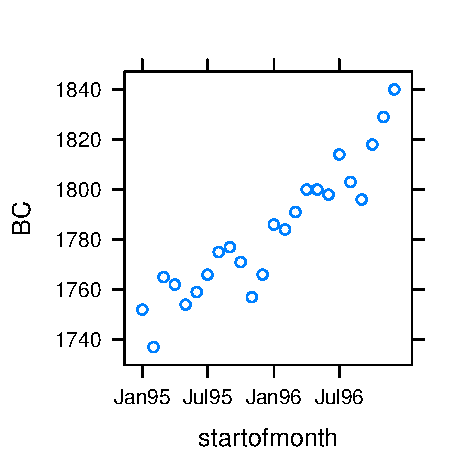
\includegraphics[width=0.97\textwidth]{figs/04-date-labs-1} }

\end{Schunk}
 \caption{Canadian worker force numbers, with dates used to label the
   $x$-axis. See Figure \ref{fig:jobsplot} in
   Subsection \ref{ss:latticeParam} for data from all Canadian
 provinces.}\label{fig:simplatparam}
\end{marginfigure}
\begin{Schunk}
\begin{Sinput}
## Labeling of graph: data frame jobs (DAAG)
library(DAAG); library(lattice)
fromdate <- as.Date("1Jan1995", format="%d%b%Y")
startofmonth <- seq(from=fromdate, by="1 month",
                    length=24)
atdates <- seq(from=fromdate, by="6 month",
               length=4)
xyplot(BC ~ startofmonth, data=jobs,
       scale=list(x=list(at=atdates,
                         labels=format(atdates,
                                       "%b%y"))))
\end{Sinput}
\end{Schunk}
%$

\paragraph{Conversion of dates to and from integer number of days:}
By default, dates are stored in integer numbers of days.  Use
\txtt{julian()} to convert a date into its integer value, by default
using January 1 1970 as origin.  Use the argument \txtt{option}
to specify some different origin:
\begin{Schunk}
\begin{Sinput}
dates <- as.Date(c("1908-09-17", "1912-07-12"))
julian(dates)
\end{Sinput}
\begin{Soutput}
[1] -22386 -20992
attr(,"origin")
[1] "1970-01-01"
\end{Soutput}
\begin{Sinput}
julian(dates, origin=as.Date("1908-01-01"))
\end{Sinput}
\begin{Soutput}
[1]  260 1654
attr(,"origin")
[1] "1908-01-01"
\end{Soutput}
\end{Schunk}

Note also \txtt{weekdays()}, \txtt{months()}, and \txtt{quarters()}:
\begin{Schunk}
\begin{Sinput}
dates <- as.Date(c("1908-09-17", "1912-07-12"))
weekdays(dates)
\end{Sinput}
\begin{Soutput}
[1] "Thursday" "Friday"  
\end{Soutput}
\begin{Sinput}
months(dates)
\end{Sinput}
\begin{Soutput}
[1] "September" "July"     
\end{Soutput}
\begin{Sinput}
quarters(dates)
\end{Sinput}
\begin{Soutput}
[1] "Q3" "Q3"
\end{Soutput}
\end{Schunk}

\paragraph{Regular sequences of dates:}  Use the function \txtt{help(seq.Date)}.

Given a vector of `event' times, the following function can be used to
count the number of events in each of a regular sequence of time
intervals:
\begin{fullwidth}

\begin{Schunk}
\begin{Sinput}
intervalCounts <- function(date, from=NULL, to=NULL, interval="1 month"){
  if(is.null(from))from <- min(date)
  if(is.null(to))to <- max(date)
  dateBreaks <- seq(from=from, to=to, by=interval)
  dateBreaks <- c(dateBreaks, max(dateBreaks)+diff(dateBreaks[1:2]))
  cutDates <- cut(date, dateBreaks, right=FALSE)
  countDF <- data.frame(Date=dateBreaks[-length(dateBreaks)],
                        num=as.vector(table(cutDates)))
  countDF
}
\end{Sinput}
\end{Schunk}

\end{fullwidth}

The following counts the number of events by year:
\begin{fullwidth}
\small

\begin{Schunk}
\begin{Sinput}
dates <- c("1908-09-17", "1912-07-12", "1913-08-06", "1913-09-09", "1913-10-17")
dates <- as.Date(dates)
(byYear <- intervalCounts(dates, from=as.Date("1908-01-01"), interval='1 year'))
\end{Sinput}
\begin{Soutput}
        Date num
1 1908-01-01   1
2 1909-01-01   0
3 1910-01-01   0
4 1911-01-01   0
5 1912-01-01   1
6 1913-01-01   3
\end{Soutput}
\end{Schunk}

\end{fullwidth}

\paragraph{Further useful functions for working with dates:}
Note
\marginnote{The CRAN Task View for Time Series Analysis has notes on
  classes and methods for times and dates, and on
  packages that give useful functionality} also \txtt{date()}
which returns the current date and time, and \txtt{Sys.Date()} which
returns the date.  For information on functions for working with
times, see \margtt{help(ISOdatetime)}.

\subsection{Summaries of Information in Data Frames}

A common demand is to obtain a tabular summary of information in each
of several columns of a data frame, broken down according to the
levels of one or more grouping variables.  Consider the data frame
\txtt{nswdemo} ({\em DAAG}). Treatment groups are control
(\txtt{trt==0}) and treatment (\txtt{trt==1}) group, with variables
\txtt{re74} (1974 income), \txtt{re75} (1975) and \txtt{re78} (1978),

The following calculates the number of zeros for each of the three
variables, and for rach of the two treatment categories:
\marginnote[12pt]{The data frame is split according to the grouping elements
specified in the \txtt{by} argument.  The function is then
applied to each of the columns in each of the splits.}

\begin{Schunk}
\begin{Sinput}
## Define a function that counts zeros
countzeros <- function(x)sum(!is.na(x) & x==0)
aggregate(nswdemo[, c("re74", "re75", "re78")],
          by=list(group=nswdemo$trt),
          FUN=countzeros)
\end{Sinput}
\begin{Soutput}
  group re74 re75 re78
1     0  195  178  129
2     1  131  111   67
\end{Soutput}
\end{Schunk}

Now find the proportion, excluding \txtt{NA}s, that are zero.
The result will be printed out with improved labeling of the rows:
\begin{Schunk}
\begin{Sinput}
## countprop() counts proportion of zero values
countprop <- function(x){
    sum(!is.na(x) & x==0)/length(na.omit(x))}
prop0 <-
  aggregate(nswdemo[, c("re74","re75","re78")],
            by=list(group=nswdemo$trt),
            FUN=countprop)
## Now improve the labeling
rownames(prop0) <- c("Control", "Treated")
round(prop0,2)
\end{Sinput}
\begin{Soutput}
        group re74 re75 re78
Control     0 0.75 0.42 0.30
Treated     1 0.71 0.37 0.23
\end{Soutput}
\end{Schunk}

The calculation can alternatively be handled by two calls to the
function \txtt{sapply()}, one nested within the other, thus:
\marginnote[12pt]{The argument \margtt{z} in the `in place' function
  is a data frame.  The argument \margtt{x} to \margtt{countprop()} is
  a column of a data frame.}
\begin{Schunk}
\begin{Sinput}
prop0 <-
  sapply(split(nswdemo[, c("re74","re75","re78")],
               nswdemo$trt),
         FUN=function(z)sapply(z, countprop))
round(t(prop0), 2)
\end{Sinput}
\begin{Soutput}
  re74 re75 re78
0 0.75 0.42 0.30
1 0.71 0.37 0.23
\end{Soutput}
\end{Schunk}
% $

\section{*Classes and Methods (Generic Functions)}\label{sec:generic}

\fbox{\parbox{\linewidth}{{\bf Key language constructs:}\\[4pt]
\begin{tabular}{ll}
Classes & Classes make generic functions (methods) possible.\\[6pt]
Methods & Examples are \txtt{print()}, \txtt{plot()}, \txtt{summary()},
etc.\\[4pt]
\end{tabular}
}
}
\vspace*{6pt}
%

There are two implementation of classes and methods, the original S3
implementation, and the newer S4 implementation that is implemented in
the \textit{methods} package. Here, consider the simpler S3
implementation.

All objects have a class. Use the function \txtt{class()} to get this
information.

For many common tasks there are generic functions --
\txtt{print()}, \txtt{summary()}, \txtt{plot()}, etc.\ -- whose action
varies according to the class of object to which they are applied.
Thus for a data frame, \txtt{print()} calls the method
\txtt{print.data.frame()}. 
\marginnote[-24pt]{For a factor, \margtt{print()} it calls
  \txtt{print.factor()}, and so on. Ordered factors `inherit'
  the print method for factors.  For objects with no explicit print
  method, \margtt{print.default()} is called.}


To get details of the S3 methods that are available for a generic
function such as \txtt{plot()}, type, e.g.,
\txtt{methods(plot)}. To get a list of the S3 methods that are available for
  objects of class \txtt{lm}, type, e.g.,
\txtt{methods(class="lm")}

\subsection{$^*$S4 methods}\label{ss:S4}
\marginnote{Packages that use S4 classes and methods include
  \textit{lme4}, Bioconductor packages, and most of the spatial
  analysis packages.}   The S4 conventions and mechanisms extend the abilities
available under S3, build in checks that are not available with S3,
and are more conducive to good software engineering practice.

\subsection*{Example -- a spatial class}\label{ss:bubble}

\marginnote{Classes defined in the {\em sp} package are widely
used across R spatial data analysis packages.}
The {\em sp} package defines, among other possibilities, spatial data
classes \txtt{SpatialPointsDataFrame} and \txtt{SpatialGridDataFrame}.

The {\em sp} function \txtt{bubble()}, for plotting spatial measurement data,
accepts a spatial data object as argument.\sidenote{Each point (location)
is shown as a bubble, with area proportional to a value for that point.}
The function \txtt{coordinates()} can be used, given spatial coordinates,
to turn a data frame or matrix into an object of one of the requisite
classes.

Data from the data frame \txtt{meuse}\sidenote{Data are from the
floodplain of the river Meuse, in the Netherlands.  It includes
concentrations of various metals (\margtt{cadmium}, \margtt{copper},
\margtt{lead}, \margtt{zinc}), with Netherlands topographical map
coordinates.}, from the \textit{sp} package, will be used for an
example.  A first step is to create an object of one of the classes
that the function \txtt{bubble()} accepts as argument, thus:
\begin{Schunk}
\begin{Sinput}
library(sp)
data(meuse)
class(meuse)
\end{Sinput}
\begin{Soutput}
[1] "data.frame"
\end{Soutput}
\begin{Sinput}
coordinates(meuse) <- ~ x + y
class(meuse)
\end{Sinput}
\begin{Soutput}
[1] "SpatialPointsDataFrame"
attr(,"package")
[1] "sp"
\end{Soutput}
\end{Schunk}
\noindent
This has created an object of the class \txtt{SpatialPointsDataFrame}.
\begin{marginfigure}[-15pt]
\vspace*{-9pt}
\begin{Schunk}


\centerline{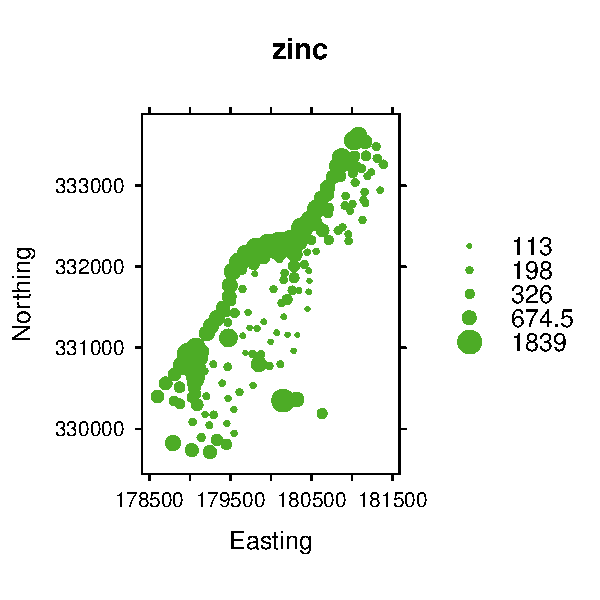
\includegraphics[width=\textwidth]{figs/04-bubble-1} }

\end{Schunk}
\caption{Bubble plot for \txtt{zinc} concentrations.  Areas of
  bubbles are proportional to concentrations.\label{fig:Znbubble}}
\end{marginfigure}
Code that creates the plot, shown in Figure \ref{fig:Znbubble}, is:
\begin{Schunk}
\begin{Sinput}
bubble(meuse, zcol="zinc", scales=list(tck=0.5),
       maxsize=2, xlab="Easting", ylab="Northing")
\end{Sinput}
\end{Schunk}
\noindent
The function \txtt{bubble()} uses the abilities of the \txtt{lattice}
package.  It returns a \txtt{trellis} graphics object.

The coordinates can be extracted using \txtt{coordinates(meuse)}.
Remaining columns from the original data frame are available from the
data frame \txtt{meuse@data}.

Use \txtt{slotNames()} to examine the structure of the object:
\begin{Schunk}
\begin{Sinput}
slotNames(meuse)
\end{Sinput}
\begin{Soutput}
[1] "data"        "coords.nrs"  "coords"     
[4] "bbox"        "proj4string"
\end{Soutput}
\end{Schunk}
\marginnote[12pt]{Note that \margtt{meuse@data} is shorthand for
  \margtt{slot(meuse, "data")}.}  Typing \txtt{names(meuse)} returns
the column names for the \txtt{data} slot.  The effect is the
same as that of typing \txtt{names(meuse@data)}.  To get a list of the
S4 methods that are available for a generic function, use
\txtt{showMethods()}. Section \ref{sec:s4} has further details.

\section{Common Sources of Surprise or Difficulty}\label{sec:difficult}
\begin{itemize}
\item[] Character vectors, when incorporated as columns of a data frame,
become by default factors.

\item[] Factors can often be treated as vectors of text strings, with
values given by the factor levels. Watch however for contexts where
the integer codes are used instead.

\item[] Use \txtt{is.na()} to check for missing values.  Do not try
  to test for equality with \txtt{NA}.  Refer back to Section
  \ref{ss:NA}.

\item[] If there is a good alternative, avoid the attaching of data
  frames.  \marginnote{Assignment of new values to an attached data
    frame creates a new local data frame with the same name.  The new
    local copy remains in the workspace when the data frame is
    detached.} If you do use this mechanism, be aware of the traps.

\item[] The syntax \txtt{elasticband[,2]}, extracts the second
  column from the data frame \txtt{elasticband}, yielding a numeric
  vector.  Observe however that \txtt{elasticband[2, ]} yields a
  data frame, rather than the numeric vector that the user may
  require.  Use the function \txtt{unlist()} to extract the vector
of numeric values.
\end{itemize}

\section{Summary}
\begin{itemize}
\item[] Important R data structures are vectors, factors, data frames and
  lists.  Vector modes include numeric, logical, character or complex.

\item[] Factors, used for categorical data, can be important in the use
  of many of R's modeling functions. Ordered factors are appropriate
for use with ordered categorical data.

\item[] Use \txtt{table()} for tables of counts, and \txtt{xtabs()}
for tables of counts or totals.

\item[] R allows the use of infinite Values (\txtt{Inf} or
  \txtt{-Inf}) and \txtt{NaN}s (not a number) in calculations.
  Introduce such quantities into your calculations only if you
  understand the implications.

\item[] A matrix is a vector that is stacked column upon column into a
  rectangular array that has dimensions given by its dimension
  attribute.  A data frame is, by contrast, a list of columns.

\item[] \marginnote[11pt]{Calculations with matrices are likely to be much
    faster than with data frames.}
Matrices are in some (not all) contexts handled similarly to data
  frames whose elements are all of one type (typically all numeric).

\item[] Lists are ``non-atomic'' vectors. Use the function
  \txtt{c()} (concatenate) to join lists, just as for ``atomic''
  vectors.

\item[] Modeling functions
\marginnote{Generic functions that
  may be used with model objects typically include
  \margtt{print()}, \margtt{summary()}, \margtt{fitted()},
\margtt{coef()} and \margtt{resid()}.} typically output a
\textit{model object} that has a list structure.  This holds
information from the model fit, in a form from which generic model
functions can then extract commonly required forms of output.

\end{itemize}

\section{Exercises}\label{sec:objects-ex}


\begin{enumerate}

\item  Find an R function that will sort a vector. Give an example.

\item  Modify the function \txtt{mean.and.sd()} so that it outputs,
in addition to mean and standard deviation, the number of
vector elements.

\item $^*$What is the mode of: (i) a factor; (ii) a dataframe?;
(iii) a list that is not necessarily a dataframe?
Apply the function \txtt{mode()} to objects of each
of these classes.  Explain what you find.

\item The attempt to assign values to an expression whose
subscripts include missing values generates an error.
Run the following code and explain the error that results:
\begin{Schunk}
\begin{Sinput}
y <- c(1, NA, 3, 0, NA)
y[y > 0]
y[y > 0] <- c(11, 12)
\end{Sinput}
\end{Schunk}

\item Run the following code:
\begin{fullwidth}

\begin{Schunk}
\begin{Sinput}
gender <- factor(c(rep("female", 91), rep("male", 92)))
table(gender)
gender <- factor(gender, levels=c("male", "female"))
table(gender)
gender <- factor(gender, levels=c("Male", "female")) # Note the mistake
                            # The level was "male", not "Male"
table(gender)
rm(gender)                  # Remove gender
\end{Sinput}
\end{Schunk}

\end{fullwidth}
The output from the final \verb!table(gender)! is

\begin{Schunk}
\begin{Soutput}
gender
  Male female 
     0     91 
\end{Soutput}
\end{Schunk}
Explain the numbers that appear.

\item In the data set \texttt{nswpsdi1} (\texttt{DAAGxtras}), do
the following for each of the two levels of \texttt{trt}:
\begin{enumerate}
  \item Determine the numbers for each of the levels of \texttt{black};
  \item Determine the numbers for each of the levels of \texttt{hispanic};
  item Determine the numbers for each of the levels of \texttt{marr} (married).
\end{enumerate}

\item Sort the rows in the data frame \texttt{Acmena} in order
of increasing values of \texttt{dbh}.\newline
[Hint: Use the function \texttt{order()}, applied to \texttt{age} to
determine the order of row numbers required to sort rows in
increasing order of age.  Reorder rows of \texttt{Acmena} to appear
in this order.]

\begin{Schunk}
\begin{Sinput}
Acmena <- subset(rainforest, species=="Acmena smithii")
ord <- order(Acmena$dbh)
acm <- Acmena[ord, ]
\end{Sinput}
\end{Schunk}

Sort the row names of \texttt{possumsites} (\textit{DAAG}) into
alphanumeric order.  Reorder the rows of \texttt{possumsites} in order
of the row names.

\item \begin{enumerate}
\item Create a \texttt{for} loop that, given a numeric vector,
  prints out one number per line, with its square and cube alongside.
\item Look up \texttt{help(while)}.  Show how to use a \texttt{while}
  loop to achieve the same result.
\item Show how to achieve the same result without the use of an explicit
loop.
\end{enumerate}
\item Here are examples that illustrate the use of \txtt{paste()}
and \txtt{paste0()}:
\begin{Schunk}
\begin{Sinput}
paste("Leo", "the", "lion")
paste("a", "b")
paste0("a", "b")
paste("a", "b", sep="")
paste(1:5)
paste(1:5, collapse="")
\end{Sinput}
\end{Schunk}
What are the respective effects of the parameters \texttt{sep} and
\texttt{collapse}?
\item The following function calculates the mean and standard deviation of a
numeric vector.
\begin{Schunk}
\begin{Sinput}
meanANDsd <- function(x){
    av <- mean(x)
    sdev <- sd(x)
    c(mean=av, sd = sdev) # The function returns this vector
}
\end{Sinput}
\end{Schunk}
Modify the function so that: (a) the default is to use \texttt{rnorm()} to
generate 20 random normal numbers, and return the standard deviation;
(b) if there are missing values, the mean and standard deviation are
calculated for the remaining values.
\item Try the following:
\begin{Schunk}
\begin{Sinput}
class(2)
class("a")
class(cabbages$HeadWt)     # cabbages is in the datasets package
class(cabbages$Cult)
\end{Sinput}
\end{Schunk}
Now do \texttt{sapply(cabbages, class)}, and note which columns hold
numerical data.  Extract those columns into a separate data frame,
perhaps named \texttt{numtinting}.\newline
[Hint: \texttt{cabbages[, c(2,3)]} is not the correct answer, but it is,
after a manner of speaking, close!]
\item Functions that may be used to get information about data
  frames include \texttt{str()}, \texttt{dim()}, \texttt{row.names()}
and \texttt{names()}. Try each of these functions with the data
  frames \texttt{allbacks}, \texttt{ant111b} and \texttt{tinting}
(all in \textit{DAAG}).

For getting information about each column of a data frame, use
\texttt{sapply()}.  For example, the following applies the function
\texttt{class()} to each column of the data frame \texttt{ant111b}.
\begin{Schunk}
\begin{Sinput}
library(DAAG)
sapply(ant111b, class)
\end{Sinput}
\end{Schunk}
For columns in the data frame \texttt{tinting} that are factors, use
\texttt{table()} to tabulate the number of values for each level.
\end{enumerate}
%
